\documentclass[wsdraft]{ws-procs11x85}

\usepackage{ws-procs-thm}
\usepackage{multirow}
\usepackage{tabularx}
\usepackage[usenames, dvipsnames]{color}
\usepackage[final]{pdfpages}

\newcommand{\etal}{\textit{et al}.}
\newcommand{\TEtranscripts}{\texttt{TEtranscripts}}
\newcommand{\SalmonTE}{\texttt{SalmonTE}}
\newcommand{\HTSeq}{\texttt{HTSeq-count}}
\newcommand{\Cuffdiff}{\texttt{Cuffdiff}}
\newcommand{\RepEnrich}{\texttt{RepEnrich}}
\begin{document}


\title{An ultra-fast and scalable quantification pipeline for transposable elements from next generation sequencing data}

\author{Hyun-Hwan Jeong$^{1,2}$, Hari Krishna Yalamanchili$^{1,2}$, Caiwei Guo$^{2,3}$, \\
Joshua M. Shulman$^{1,2,3,4}$, Zhandong Liu$^{2,5,\dag}$}

\address{$^{1}$Department of Molecular and Human Genetics, Baylor College of Medicine,\\
$^{2}$Jan and Dan Duncan Neurological Research Institute, Texas Children’s Hospital,\\
$^{3}$Department of Neuroscience, Baylor College of Medicine,\\
$^{4}$Department of Neurology, Baylor College of Medicine,\\
$^{5}$Department of Pediatrics, Baylor College of Medicine,\\
Houston, Texas 77030, USA\\
$^{\dag}$E-mail: zhandonl@bcm.edu}

\begin{abstract}

Transposable elements (TEs) are DNA sequences which are capable of moving from one location to another and represent a large proportion (45\%) of the human genome. 
TEs have functional roles in a variety of biological phenomena such as cancer,
neurodegenerative disease, and aging.
Rapid development in RNA-sequencing technology has enabled us, for the first time, to study the activity of TE at the systems level.  


However, efficient TE analysis tools are not yet developed.
In this work, we developed \SalmonTE, a fast and reliable pipeline for the quantification of TEs from 
RNA-seq data.
We benchmarked our tool against \TEtranscripts, a widely used TE quantification method,  and three other quantification methods using several RNA-seq datasets from
Drosophila melanogaster and human cell-line.
We achieved 20 times faster execution speed without compromising the accuracy.
This pipeline will enable the biomedical research community to quantify and analyze TEs from large amounts of data and lead to novel TE centric discoveries.


\end{abstract}

\keywords{Transposable Element; Quasi-Mapping; RNA-seq; Next Generation Sequencing; Large Scale Genome Analysis}

\copyrightinfo{\copyright\ 2017 The Authors. Open Access chapter published by World Scientific Publishing Company and distributed under the terms of the Creative Commons Attribution Non-Commercial (CC BY-NC) 4.0 License.}

\bodymatter

\section{Introduction}\label{aba:intro}

Transposable elements (TEs) are DNA elements which can be mobilized or inserted into the genome and represent a significant proportion of most eukaryotic genomes \cite{erwin2014mobile}. 
Most of the TEs in the genome are not functional and had been considered as `junk DNA,' except for a few that retain intact functions such as transcription and mobilization.\cite{biemont2006genetics}
Furthermore, the mobilization of TEs can disrupt normal gene structure in the genome, sometimes leading to disease such as cancer \cite{belancio2008mammalian,jirtle2007environmental} neurodegenerative diseases,\cite{erwin2014mobile} and aging.\cite{wood2013chromatin} 

Recent development of high-throughput Next Generation Sequencing (NGS) technologies, like RNA-seq, enables genome-wide study for TEs \cite{ohtani2013dmgtsf1,mihevc2016tdp,li2012transposable,krug2017retrotransposon}. Toward this end, several algorithms and pipelines were proposed to analyze reads files from TE studies \cite{lee2012landscape,platzer2012te,helman2014somatic,henaff2015jitterbug,jin2015tetranscripts,de2017identifying,tang2017human}. However, most of the tools share some common limitations: 1) discordant read mapping due to increased chance of multiple mapping in repetitive elements from TEs in the same clade, 2) limited scalability for large-scale analysis, and 3) small coverage for the entire TEs defined in the human genome, i.e., a tool used in [\refcite{tang2017human}] only considered LINE 1 (Long Interspersed Nuclear Element 1) elements.\cite{ewing2015transposable} 

Among the existing tools, \TEtranscripts~has performed well on various datasets.\cite{jin2015tetranscripts}
Nonetheless, The scalability of \TEtranscripts~is a critical limiting factor for large systems biology studies because it cannot handle \verb|FASTQ| files directly and needs \verb|SAM| (Sequence Alignment Map)/\verb|BAM| (Binary Sequence Alignment Map) files generated from raw \verb|FASTQ| files. Since there are many tuning parameters on handling repetitive sequence among different RNA-seq mapping algorithms, this step will be highly variable depending on the mapping parameters and sometimes even generate artifactual results if a unique mapping parameter is superimposed by a previous analyst who handled the mapping. 

Although \TEtranscripts~is the fastest tool for TE quantification \cite{jin2015tetranscripts}, the interval tree algorithm \cite{samet1990design}, which is used to find the interval of genes or TEs on the reference genome,  performed poorly in terms of running time in practice, making \TEtranscripts~suboptimal for large-scale TE analysis.

In recent studies,  many large-scale analysis of public meta RNA-seq datasets offered new insight and findings that cannot be discovered in each dataset alone. \cite{nellore2016human} However, a meta-study on TE without using a large number of high-performance computing cluster is not yet feasible given the time complexity of current algorithms.  Toward this end, we developed a new pipeline called \SalmonTE. It deploys a low time-complexity quantification method, \verb|Salmon|\cite{patro2017salmon}, and contains various statistical models for TEs quantification. Moreover, \SalmonTE~provides a rich set of built-in functions for data pre-processing from raw \verb|FASTQ| files. 
In the results section, we demonstrate the running speed of \SalmonTE~outperforms all other methods including \TEtranscripts~ and delivers a reliable quantification result as well.

\section{Methods}

The proposed pipeline consists of three parts: library preparation, quantification, and statistical analysis (Figure \ref{aba:fig1}). To increase the usability and to enable parallel processing for multiple RNA-seq reads files, we adopted the \texttt{Snakemake} workflow system and wrote a script based on the execution rule of \texttt{Snakemake} for the TE quantification.\cite{koster2012snakemake} In contrast to TEtranscripts, SalmonTE starts with raw RNA-seq files, and does not need any additional pre-processing for a given sequence file. Moreover, TEtranscripts requires a modified GTF files based on RepeatMasker database.\cite{RepeatMasker} SalmonTE only needs the FASTA file of cDNA (complementary DNA) sequences of each TE. The entire source code and executable scripts are available at \url{https://github.com/hyunhwaj/SalmonTE}.

\begin{figure}[h]
\centerline{
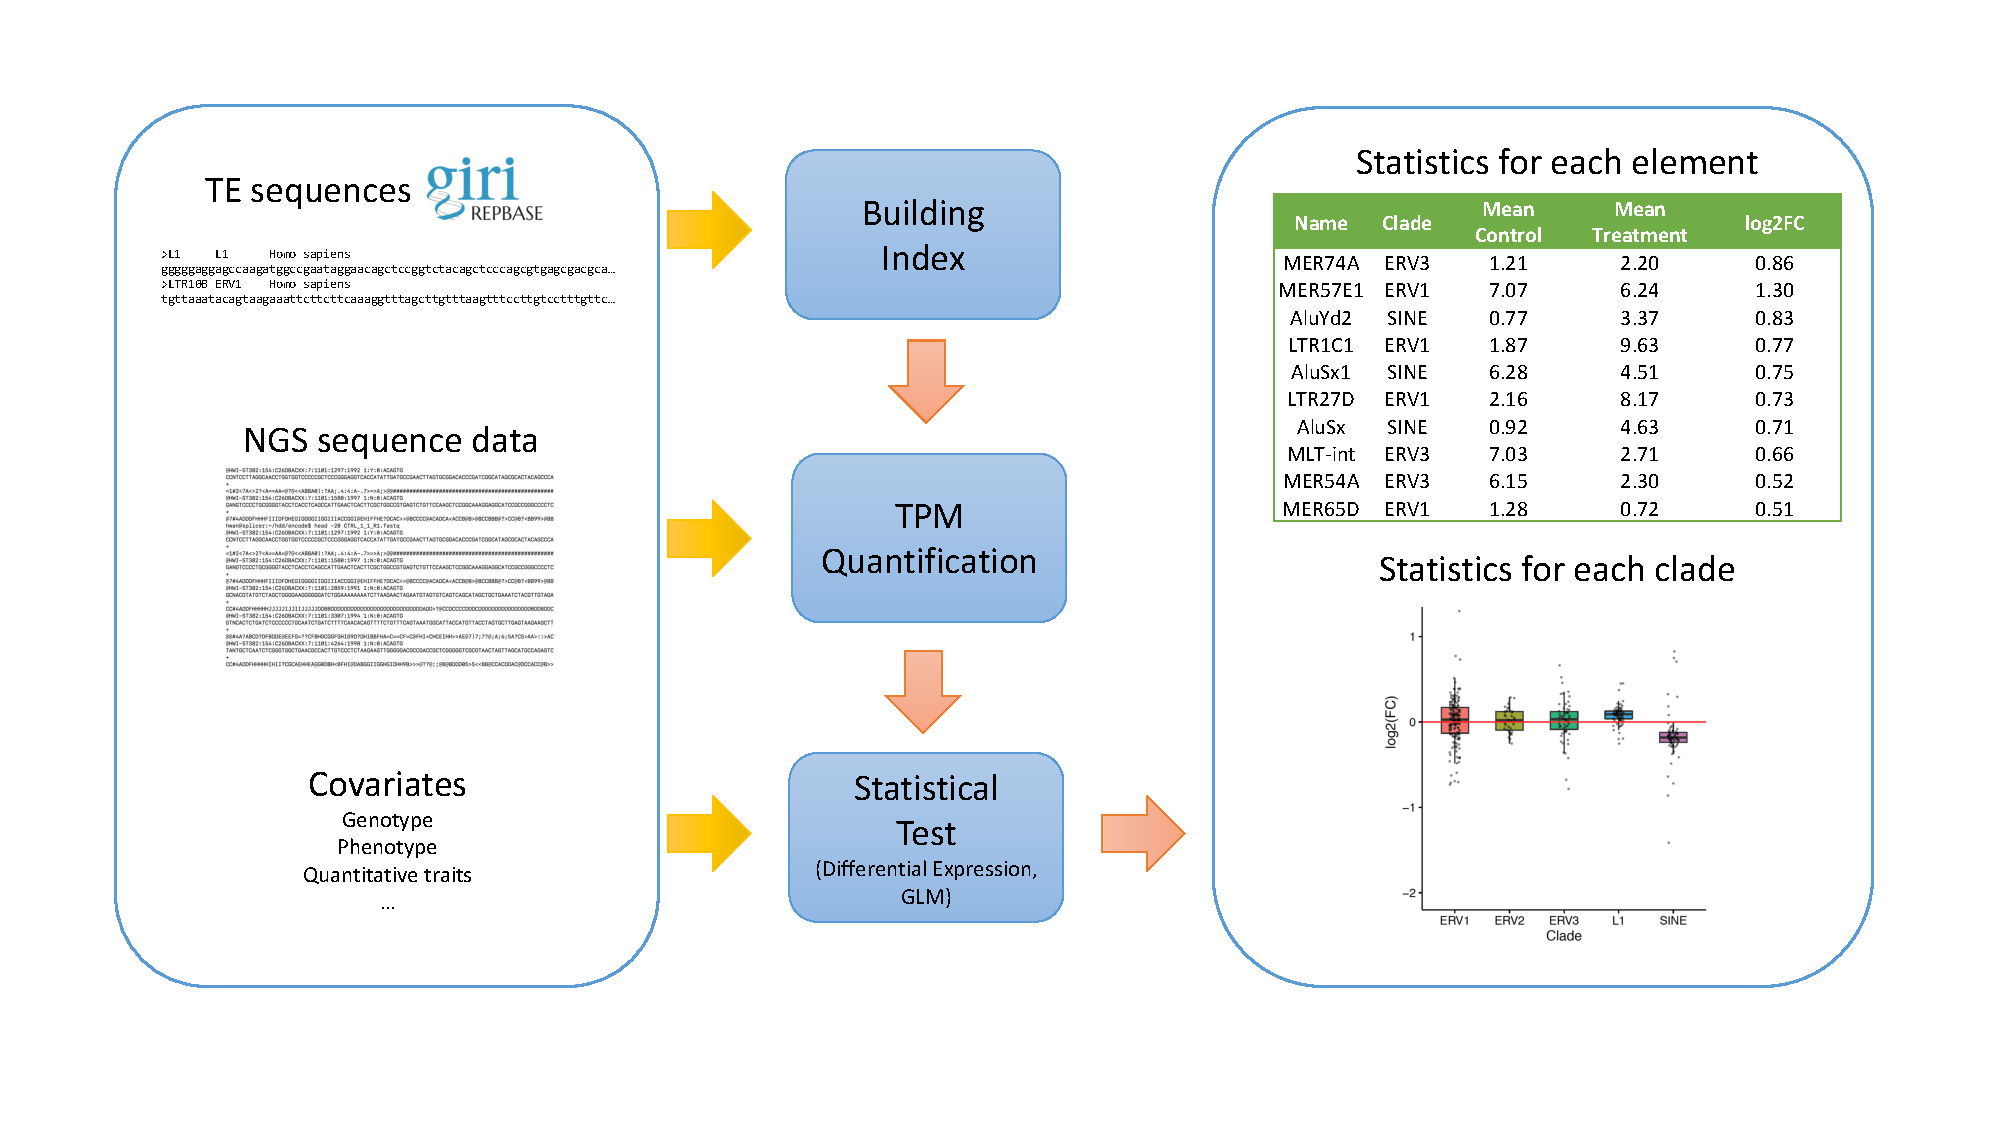
\includegraphics[width=14cm]{fig1.pdf}
}
\caption{An illustration of the \SalmonTE~pipeline. Left Panel: Input from Repbase to build the mapping index, raw \texttt{FASTQ} file, and covariates for statistical testing.  Middle Panel: The workflow of \SalmonTE~consists of three parts: building the index based on Repbase or user-input cDNA sequences of TEs, quantification based on \texttt{FASTQ} file, and statical test through the generalized linear model or differential expression analysis. Right Panel: Example output including the statistical report and box plot on estimated $log_2$ fold-change.}
\label{aba:fig1}
\end{figure}

\subsection{Transposable Element Library Preparation}
% revised
To build the index library for the quasi-mapping, \SalmonTE~takes the FASTA file of cDNA sequences from TE databases such as Repbase (version 22.06)\cite{repbase}. In the current version, the index files for \textit{Homo sapiens} and \textit{Drosophila melanogaster} are available. 
We reasoned that it is hard to estimate TEs which replicate without an RNA intermediate from RNA-seq sample. Therefore, we excluded the following elements: simple repeats and multi-copy genes, and DNA transposable. After collecting the cDNA sequences, we manually curated clades of each TE based on the repeat class annotation from Repbase. \\
As a result, the generated TE library index database contains 687 TEs for \textit{Homo sapiens} and 163 TEs for \textit{Drosophila melanogaster}.

\subsection{Salmon quantification algorithm}

We adopted the \texttt{Salmon} [\refcite{patro2017salmon}] algorithm to estimate the relative TE abundance from a given RNA-seq sample. \texttt{Salmon} enables a fast and accurate quantification of TE expression from RNA-seq reads with a light-weight mapping, online initial expression estimation phase, and offline inference for the estimation refinement.\cite{patro2017salmon,srivastava2016rapmap,bishop2006pattern,foulds2013stochastic} 
Salmon quantifies the relative abundance of each TE given a set of TE sequences $T$ and a set of sequenced fragments (reads) $F$.
Suppose that we have $M$ TEs and the set of underlying true TE counts are given as $T = \{(t_1, \dots , t_M), (c_1, \dots, c_M) \}$, where $t_i$ is the nucleotide sequence of $i$-th TE in the set and $c_i$ is the true count of the corresponding TE. If $T$ contains a complete count, we can calculate the nucleotide fraction $\eta_i$ of each $t_i$ from (\ref{eq:1}),

\begin{equation} \label{eq:1}
\eta_i = \frac{c_i \cdot \widetilde{l_i} }{\sum_{j=1}^{M} c_j \cdot \widetilde{l_j}}
\end{equation}
where $\widetilde{l_i}$ is the effective transcript length of $t_i$\cite{li2009rna}.

We can also calculate the Transcripts Per Million (TPM) using (\ref{eq:2}),

\begin{equation} \label{eq:2}
TPM_i = \frac{ \frac{\eta_i }{\widetilde{l_i}} }
{\sum_{j=1}^{M} \frac{\eta_j }{\widetilde{l_j}} }\times 10^6
\end{equation}
where $TPM_i$ is used as a relative abundance of each transposable element in a given sample. 

It is difficult to directly estimate the $\eta$ and $TPM$ given $T$ and $F$, so \texttt{Salmon} performs the following processes. First,
\texttt{Salmon} runs a quasi-mapping procedure which is initially proposed in [\refcite{srivastava2016rapmap}]. A quasi-mapping specifies the target of each given read and also determines the position and the orientation of the read concerning the target by computing the
Maximum Mappable Prefix (MMP) [\refcite{li2012exploring}] and Next Informative Position (NIP) [\refcite{srivastava2016rapmap}] of the read.
This mapping procedure uses a generalized suffix array \cite{manber1993suffix} and enables a fast and accurate mapping as compared to other mapping tools, such as \texttt{Bowtie 2}, \texttt{STAR}, and \texttt{Kalisto} \cite{srivastava2016rapmap}. The mapping also provides a possible mapping locations for each read.

The maximum-likelihood objective model for a set of reads $F$ is defined as follows:

\begin{equation} \label{eq:3}
Pr\{F|\eta,Z, T \}=
\prod_{j=1}^{N}\sum_{i=1}^{M} Pr\{ t_i | \eta \}  \cdot
 Pr \{ f_i | t_i, z_{ij}=1 \}
\end{equation}

where $z_{ij} = 1$ if $j$-th read in $F$ is derived from $i$-th TE. Since $Pr \{f_i| t_i, z_{ij}=1\}$ is unknown, \texttt{Salmon} uses the following auxiliary terms to define conditional model to estimate the probability:

\begin{equation}
Pr \{f_j | t_i \} = Pr \{ l | t_i \} 
\cdot Pr \{ p | t_i, l \} 
\cdot Pr \{ o | t_i \} 
\end{equation}

where $Pr \{ l | t_i \}$  is the probability of drawing a read of the inferred length $l$ given $t_i$,  
$Pr \{ p | t_i, l \}$ is the probability of the read starting at position $p$ on $t_i$,
$Pr \{ o | t_i \}$ is the probability of obtaining a read alignment with the given orientation $o$ to $t_i$, and this model accounts for sample-specific parameters and biases. 

With these probabilistic models, \texttt{Salmon} performs online inference to estimate read counts $\alpha$ and nucleotide fraction $\eta$ using a variant of stochastic collapsed variational Bayesian inference (See Supplementary Algorithm in [\refcite{patro2017salmon}]).\cite{foulds2013stochastic} In addition to  the inference algorithm, \texttt{Salmon} constructs equivalence classes for a given $F$. We assign any pair of reads mapped to same set of target TEs in the same equivalence class. This construction shrink the representation of the sequencing experiment and greatly reduce the running time of offline phase.\cite{patro2017salmon}

Next, \texttt{Salmon} starts the offline phase. Given the set of equivalence classes of $F$, an EM algorithm was used to refine the previous estimation for each equivalence class with following objective function $L$:

\begin{equation}
L\{\alpha| F, Z, T\} = \prod_{j=1}^{N} \sum_{i=1}^{M} \hat{\eta_i} Pr \{f_j|t_i\}
\end{equation},
where $\hat{\eta_i}=\frac{\alpha_i}{\sum_{j}\alpha_j}$. Once the offline phase is done, \texttt{Salmon}  outputs the estimation of each TE abundance for $F$.

\subsection{Statistical tests}
We provide a statistical analysis function to identify differentially expressed TEs from the counts table as the last step of the pipeline. 
Differential analysis using DESeq2 can handle  binary covariates such as binary genotype: phenotype and gender \cite{love2014moderated}. To handle quantitative covariates such as age, we apply the General Linear Model (GLM)\cite{johnston1980multivariate}. The statistical analysis will produce two statistics to represent associations between the TEs and the covariates: the first one is the test statistics for each TE, and the second one is the summary of the statistics for each clade. 
The output files are provided with various file formats, such as tab-separated values file (TSV), XML spreadsheet file format (XLS, XLSX), R object file (Rdata), and Portable Document Format (PDF) file.

\section{Results}

\subsection{Datasets}
Two datasets were used for our comparison to other methods. 
The first dataset is the RNA-seq data from Gene Expression Omnibus (accession no. GSE47006)
which includes wild-type and \textit{Piwi} (P-element Induced WImpy testis) knockdown flies. This dataset was used as a benchmark dataset in the \TEtranscripts~paper as well.\cite{ohtani2013dmgtsf1} We compared the performance in terms of running time and quantification accuracy between our proposed pipeline and other tools, including \TEtranscripts, \HTSeq, \Cuffdiff~and \RepEnrich.\cite{jin2015tetranscripts,anders2015htseq,trapnell2013differential,criscione2014repenrich}

In the second dataset, we seek to identify new TEs that are associated with Amyotrophic Lateral Sclerosis (ALS). 
We  applied our pipeline to a K562 cell-line RNA-seq dataset from ENCODE (Encyclopedia of DNA Elements, \url{http://encodeproject.org})  Consortium (accession ID: ENCBS555BYH).\cite{encode2012integrated}
The dataset consists of two biological replicates of shRNA (short hairpin RNA) knockdown (KD) targeting \textit{TARDBP} (TAR DNA Binding Protein, as known as TDP-43) gene and two biological replicates of controls (a shRNA inserted but targets no genes). 
It has been reported that loss of \textit{TDP-43} function causes  ALS.\cite{yang2014partial,mihevc2016tdp} To measure scalability with the dataset. we also ran \TEtranscripts~to compare running time of both methods. We also performed an integrative analysis for highly differentially expressed TEs for further understanding of any new mechanism of ALS.



\subsection{Computational experiment setup}

Generating BAM files from \verb|FASTQ| files are mandatory to  \TEtranscripts, \HTSeq, \Cuffdiff, and \RepEnrich, we applied \verb|STAR| [\refcite{dobin2013star}] to generate the files with the following parameters: \verb|--outFilterMultimapNmax 100| and \verb|--–winAnchorMultimapNmax 100|. Sixteen threads were used for  both \SalmonTE~and \verb|STAR| . We also used the same parameter setup for each quantification tool similar to the \TEtranscripts~paper.

All of the computational experiments were done in a workstation with \texttt{Intel(R) Xeon(R) CPU E5-2630 v4 @ 2.20GHz} (10 cores and maximum 40 threads) and \texttt{128GBytes} RAM. 

\subsection{\SalmonTE~guarantees a reliable TE expression estimation}

For the quantification accuracy comparison, we first took estimated abundance of 8 TEs from each quantification tool. To validate the results, Reverse Transcription-quantitative Polymerase Chain Reaction (RT-qPCR) was done on these 8 TEs [\refcite{ohtani2013dmgtsf1}].
We observed \SalmonTE~outperformed all other tools ($r^2=0.98$, Figure \ref{aba:fig4} and Table \ref{aba:table_corr}). We also found that \SalmonTE~identified a weak down-regulation of DM1731\_I and HETA which was missed by \TEtranscripts.

\begin{figure}[h]
\centerline{
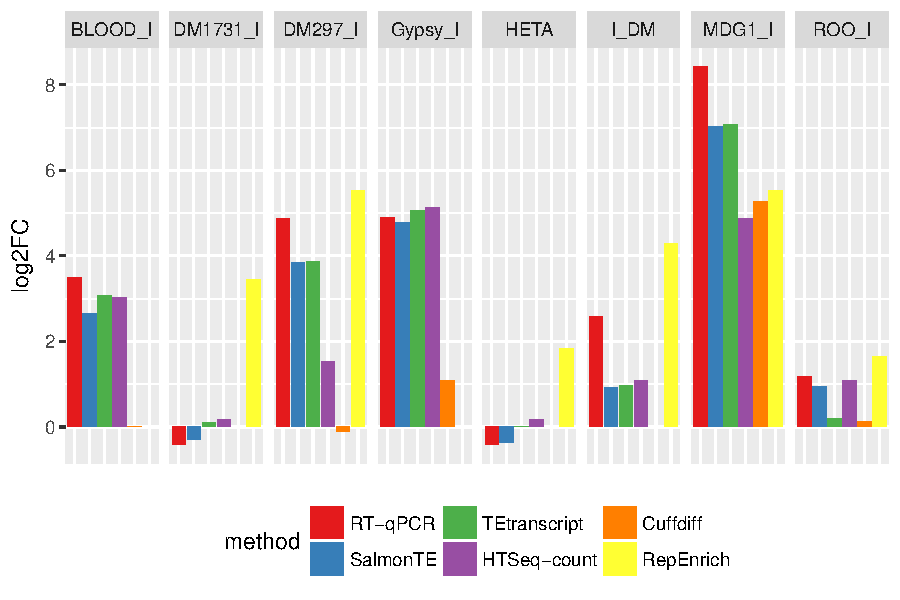
\includegraphics[width=14cm]{fig_bar}
}
\caption{Comparison of Drosophila TE expression estimation. Four computational methods were compared to \SalmonTE.  
RT-qPCR was used to validate the expression levels of the 8 TEs in the
Drosophila samples.}
\label{aba:fig4}
\end{figure}

\begin{table}[h]
\tbl{Pearson Correlation between RT-qPCR and computational TE quantification methods.}
{\begin{tabular}{l|lllll}
	\hline
	Method    & \SalmonTE & \TEtranscripts & HTSeq-count & Cuffdiff & RepEnrich  \\ \hline
	 $r^2$ & 0.98 & 0.97 & 0.85 & NA & NA \\ \hline
\end{tabular}}\label{aba:table_corr}
\end{table}

\begin{figure}[h]
\centerline{
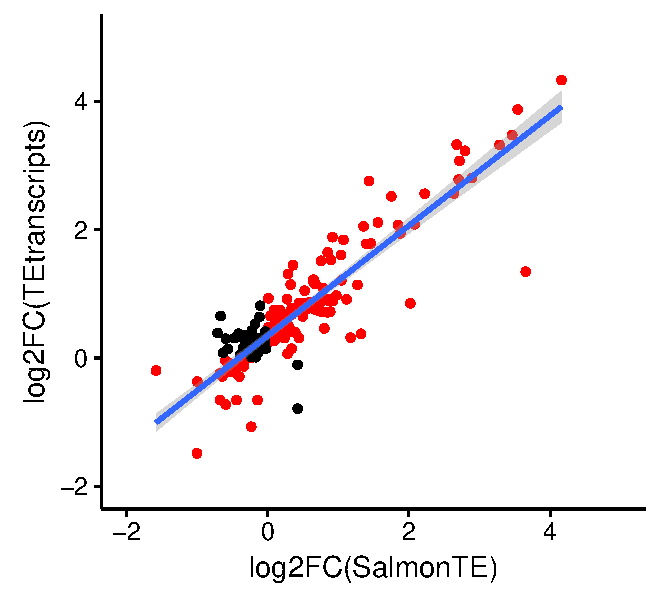
\includegraphics[width=11cm]{figure_corr_FC}
}
\caption{Correlation of $log_{2}FC$ ($\frac{Piwi}{WT}$) for each transposable element between \SalmonTE~and \TEtranscripts. Red points represent TEs with the same fold change direction between \SalmonTE~and \TEtranscripts.}
\label{aba:fig2}
\end{figure}

Next, we compared the estimated $log_{2}FC$ of \SalmonTE~ to \TEtranscripts on each transposable element for a deeper investigation. Our data shows that the estimated TE abundance of both methods are highly correlated ($r^{2}=0.98$), and we also observed there is a high concordance in the direction of fold-changes between \SalmonTE~and \TEtranscripts~(Figure \ref{aba:fig2}). We also measured the correlations of normalized read counts between \SalmonTE~and \TEtranscripts, 
and we observed that the calculated read counts from those methods are highly correlated in each sample as well ($r^2=0.92$ for wild-type (WT) sample and $r^2=0.91$ for Piwi KD sample).
From this observation, we conclude that both tools generate a similar estimation result. 
It is not a surprising result because \TEtranscripts~deploys \texttt{RSEM} algorithm,\cite{li2011rsem} and previous studies have demonstrated that transcripts count estimations from \texttt{RSEM} and \texttt{Salmon} are very correlated.\cite{jin2017comprehensive,zhang2017evaluation}

\begin{figure}[h]
\centerline{
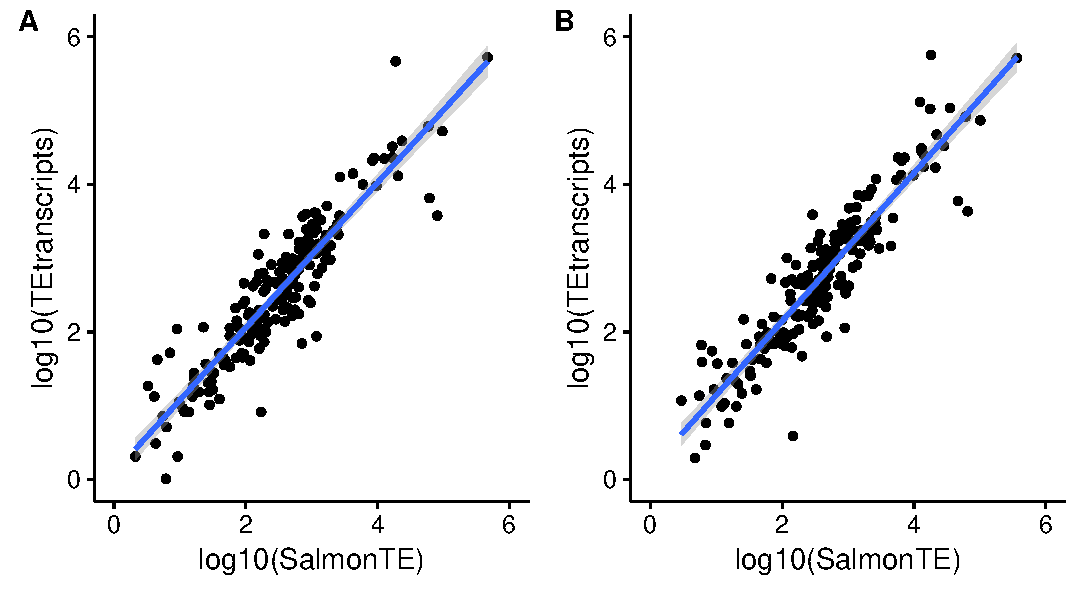
\includegraphics[width=13cm]{figure_corr_count}
}
\caption{Sample correlation of count for each transposable element between \SalmonTE~and \TEtranscripts. \textbf{A}. WT sample, \textbf{B}. Piwi KD sample.}
\label{aba:fig3}
\end{figure}



\subsection{\SalmonTE~shows a better scalability in the speed benchmark dataset}
We measured the speed of \SalmonTE~and\TEtranscripts~on two different datasets (Table \ref{aba:table1}).  
Compared to \TEtranscripts,  \SalmonTE~ showed a 19x to 27x fold increase in speed.
In this analysis, we demonstrate that \SalmonTE~outperformed \TEtranscripts~in processing speed. Our pipeline finishes in less than 5 minutes, while \TEtranscripts~needs about 2 hours to process a single sample. 
Moreover, our benchmark shows that estimated cost of our pipeline in the cloud computing environment  is for the thousands of samples 22 times cheaper than \TEtranscripts~in the computing environment (Table \ref{aba:table_amazon}).



\begin{table}[h]
\tbl{Running speed comparison between \SalmonTE~and \TEtranscripts.}
{
\begin{tabular*}{.8\textwidth}{@{\extracolsep{\fill}}llll}
\hline
Dataset                          & Piwi KD [\refcite{ohtani2013dmgtsf1}]    & K562 \textit{TDP-43} \\ \hline
Total number of samples          & 2          & 4             \\ 
RNA-seq file type                & Single end & Paired ends  \\ 
Total number of reads            & 90,411,467 & 309,701,182   \\ \hline
\SalmonTE~runtime (hh:mm:ss)      & 0:05:33    & 0:17:13       \\
\TEtranscripts~runtime (hh:mm:ss) & 1:45:26    & 7:49:40       \\
Speedup                          & 19.00x     & 27.28x        \\ \hline
\end{tabular*}}\label{aba:table1}
\end{table}

\begin{table}[h]
\tbl{Price estimation of \SalmonTE~and \TEtranscripts~in cloud computing environment (Amazon Elastic Compute Cloud (EC2),
and Amazon Elastic Block Store (EBS)). We assume that the size of a \texttt{FASTQ} file for a sample is 20GB for the calculations.}
{\begin{tabular}{lrr}
\hline
Methods & \SalmonTE~& \TEtranscripts \\ \hline
Estimated using 1000 samples & 90 hours & 2,000 hours \\ 
The price of Amazon EC2 (m4.10xlarge, US Oregon region) [\refcite{ec2}] & \$180 & \$ 4,000 \\
The price of Amazon EBS (gp2 40TB, US Oregon region) [\refcite{ebs}] & \$500 & \$ 11,111 \\  
Total price & \$680 & \$ 15,111 \\ \hline
\end{tabular}}\label{aba:table_amazon}
\end{table}

\subsection{Discover differentially expressed TEs in ALS cell line}
Next, we applied \SalmonTE~pipeline to the \textit{TDP-43} knockdown dataset.
We identified 23 transposable elements that are differential expressed between TARDBP knockdown and control cell lines (Table \ref{aba:table2}) with the threshold of $|log_{2}FC| \geq 0.5$. No statistical test were performed because the number of replicates in the dataset are small. 

We can see that most of the differentially expressed features are Endogenous Retrovirus (15 of 23) in \textit{TDP-43} cell-line sample, and we hypothesize that some of the differentially Endogenous Retrovirus TEs are associated with ALS.
\textit{TDP-43} is an established and well-studied DNA and RNA binding protein,
and could potentially regulate transposable elements at multiple levels.\cite{tan2016extensive} 
To facilitate a mechanistic understanding of the underlying regulatory mechanism of \textit{TDP-43} and to substantiate the identified differentially expressed transposable, we performed an integrative analysis by combining RNA-seq and \textit{TDP-43} binding data. 
We obtained DNA binding (ChIP-Seq [\refcite{johnson2007genome}] data) and RNA binding (CLIP-Seq [\refcite{darnell2010hits}] data)
datasets of \textit{TDP-43} in the same K562 cell line from the ENCODE consortium.
For illustration, we choose MER74A and AluJo elements that are highly up and down regulated respectively and are also found in 
Dfam database.\cite{hubley2015dfam} We quantified the number of overlapping \textit{TDP-43} ChIP/CLIP peaks with MER74A and AluJo annotations 
from Dfam. We observed that AluJo element which is down regulated in \textit{TDP-43} knockdown samples is enriched for \textit{TDP-43} 
ChIP and CLIP peaks as shown in Figure \ref{aba:fig_hari}, which might indicate that \textit{TDP-43} positively regulate AluJo elements. 
On the other hand, we did not find any enrichment of \textit{TDP-43} binding for MER74A elements. This preferential binding of \textit{TDP-43} substantiates the differentially expressed transposable elements by our pipeline. 

\begin{table}[h]
\tbl{23 Differentially expressed transposable elements in the ENCODE TARDBP data}{
\begin{tabular*}{.5\textwidth}{@{\extracolsep{\fill}}ccc}
\hline
Name & Clade & log2FC\\
\hline
MER74A & ERV3 & 1.68\\
MER57E1 & ERV1 & 1.30\\
AluYd2 & SINE & 0.83\\
LTR1C1 & ERV1 & 0.77\\
AluSx1 & SINE & 0.75\\
LTR27D & ERV1 & 0.73\\
AluSx & SINE & 0.71\\
MLT-int & ERV3 & 0.66\\
MER54A & ERV3 & 0.52\\
MER65D & ERV1 & 0.51\\
LTR28 & ERV1 & -0.59\\
LTR1F & ERV1 & -0.63\\
FLAM & SINE & -0.64\\
MER21 & ERV3 & -0.68\\
MER101 & ERV1 & -0.69\\
LTR26B & ERV1 & -0.70\\
MER83C & ERV1 & -0.71\\
AluJo & SINE & -0.72\\
LTR06 & ERV1 & -0.73\\
MLT2D & ERV3 & -0.78\\
AluYf5 & SINE & -0.86\\
AluYd3 & SINE & -1.41\\
THER2 & SINE & -2.03\\ \hline
\end{tabular*}}\label{aba:table2}
\end{table}

\begin{figure}[h]
\centerline{
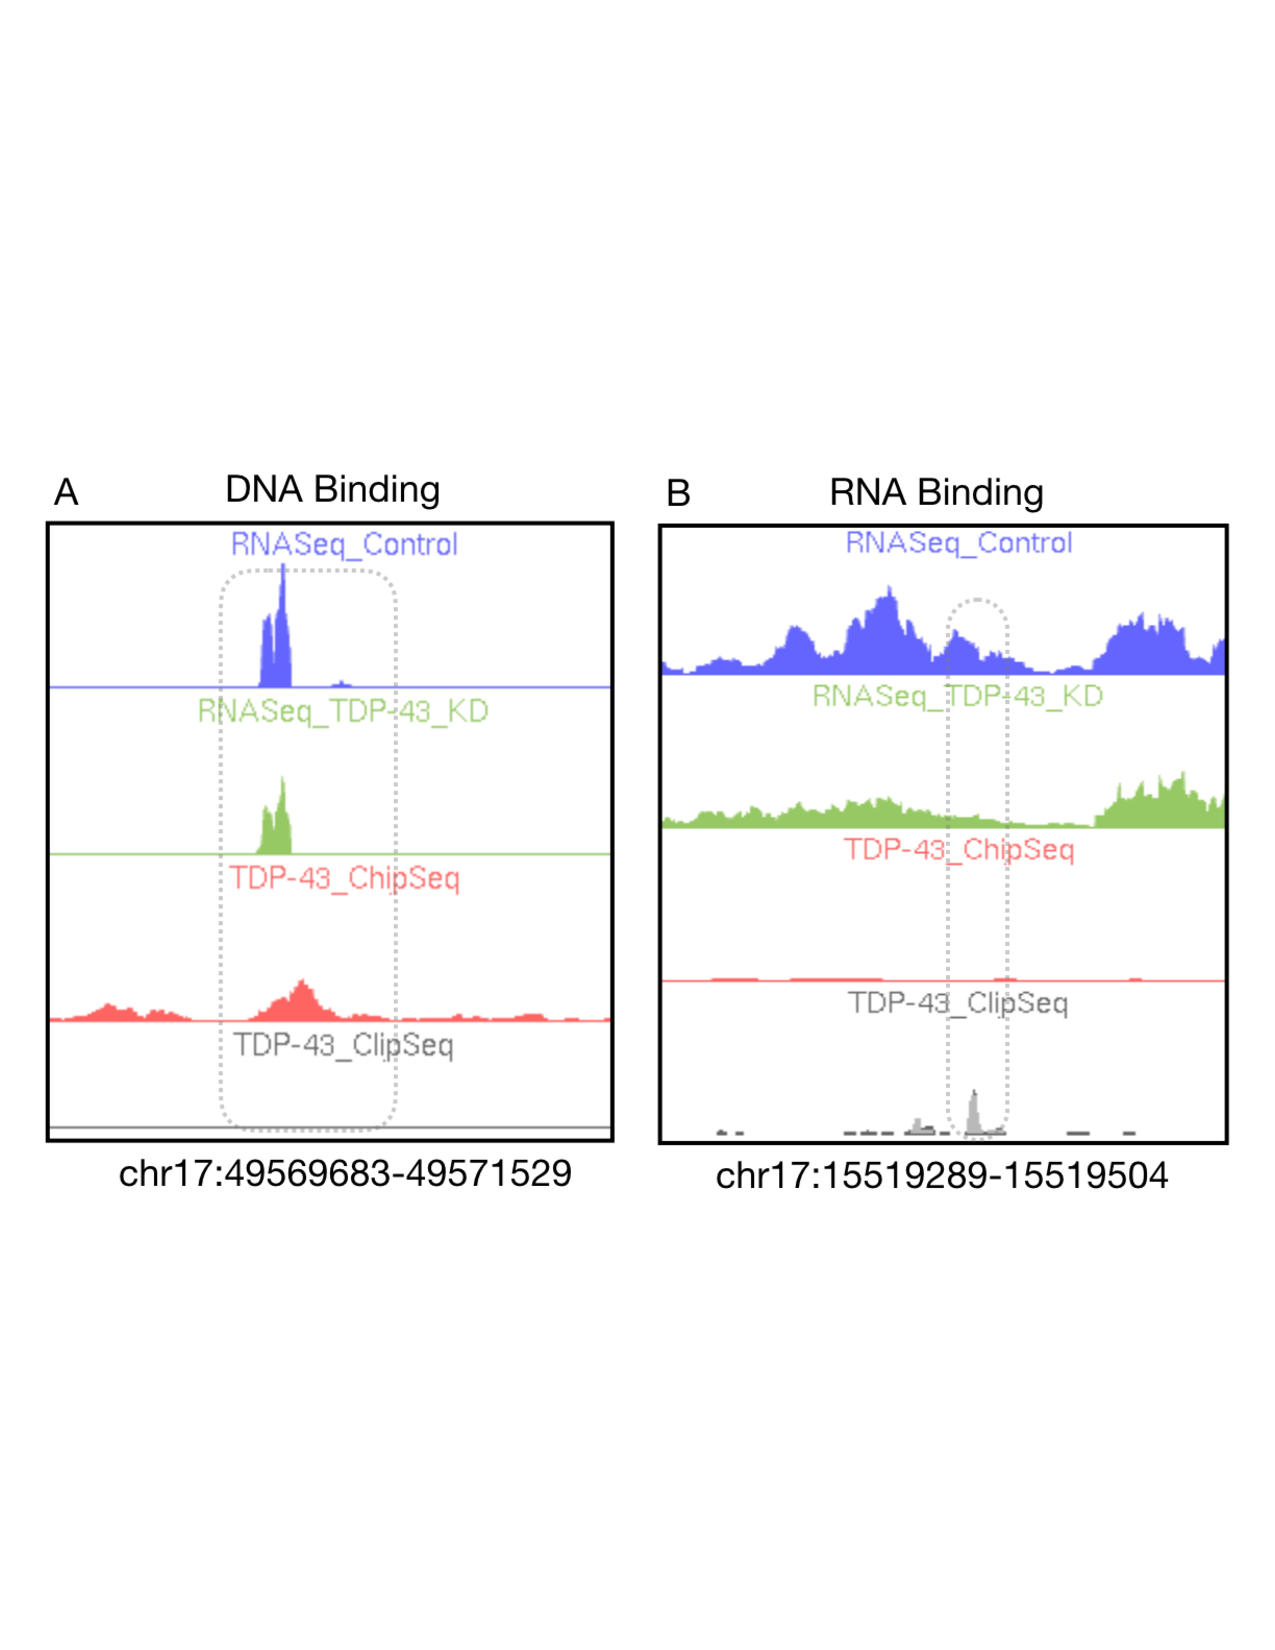
\includegraphics[width=16cm]{fig_hari}
}
\caption{
\textbf{A}. Showing down-regulation of AluJo with \textit{TDP-43} ChIP-seq peak,
\textbf{B}. Showing down-regulation of AluJo with \textit{TDP-43} CLIP-seq peak.
}
\label{aba:fig_hari}
\end{figure}


To identify if there is any general differential expression trend on subfamilies of TEs, we grouped all the TEs based on their clade information. We excluded all of the CR1 (Chicken Repeat 1) since the number of such elements in the clade is small.
We found that SINE (Short Interspersed Nuclear Elements) are mostly down expressed,
and elements in L1 (Long interspersed nuclear element 1) are generally over expressed in \textit{TDP-43} knockdown samples. 
This result provides a working hypothesis that knocking-down of \textit{TDP-43}  repress the expression of SINE elements and induce the expression of L1 elements.

\begin{figure}[h]
\centerline{
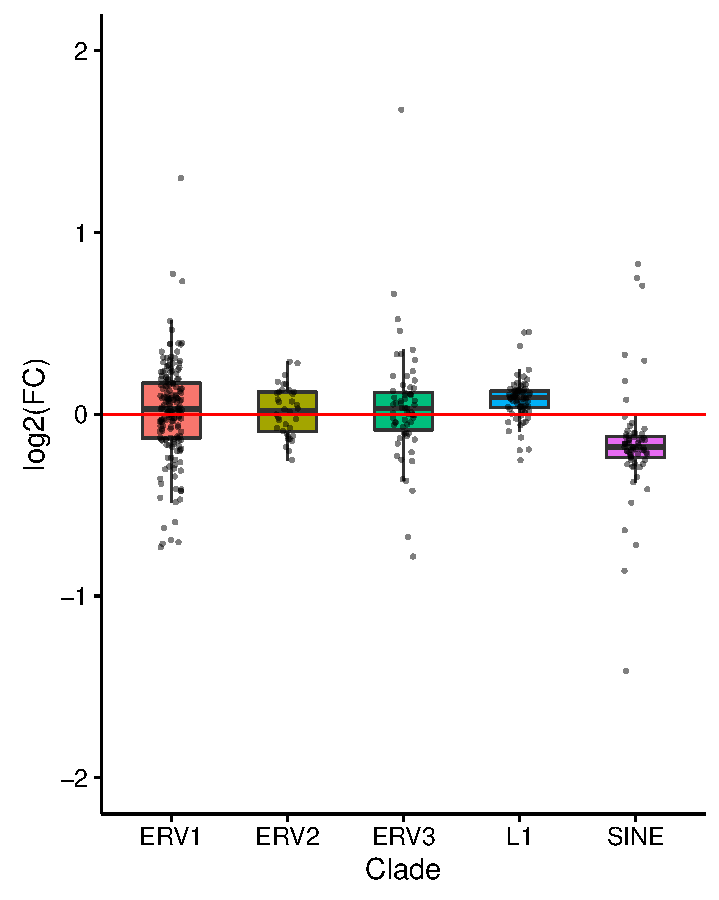
\includegraphics[width=8cm]{boxplot-clade-k562}
}
\caption{A boxplot of $log_{2}FC$ for each clade in the ENCODE \textit{TDP-43} data}
\label{aba:fig5}
\end{figure}

\section{Conclusion}


In this work, we developed \SalmonTE, a fast and reliable pipeline for quantification of TEs from 
NGS data.
Our results of \SalmonTE~on the various datasets have shown a large speed-up in computing time relative to \TEtranscripts, 
while preserving an accurate quantification on TEs. 
Therefore, we expect this pipeline will enable the biomedical research community to rapidly quantify and analyze TEs from large amounts of data generated over the past years that are otherwise lost due to genome-masking. Our tool could help the research community to discovery many TE associated with diseases.

There are still several remaining features that could be implemented in the future to improve the usability of \SalmonTE. 
For example, prediction of genomic locations, which contain the differentially expressed TEs, is useful in many TE studies. Several methods were developed toward this end\cite{de2017identifying,criscione2014transcriptional}, but these tools share the scalability issue and require massive computing power for a large-scale TE study. 
Moreover, alignment free algorithms are intrinsically limited to addressing this question. 
Therefore, we foresee a novel algorithm which extends and improves the current alignment-free methods.

\section*{Acknowledgments}
This work has been supported by National Institute of General Medical Sciences R01-GM120033, National Science Foundation - Division of Mathematical Sciences DMS-1263932, Cancer Prevention Research Institute of Texas RP170387, Houston Endowment (Z.L.), and the Alzheimer's Association (J.M.S.). 
We thank Kala Pham and Rami Al-Ouran for comments that greatly improved this manuscript.


\bibliographystyle{ws-procs11x85}
\bibliography{ws-pro-sample}

\end{document}
